% ============================================================
%  第五卷 第十一章 甚高密度物质的性质（§106–§109）
%  底本：高教社中文版第5版（束仁贵/束莼 译，郑伟谋 校）
%  OCR 底稿 full_merged.md 行 10990–11514；对照 原书转换/pages/p-293…p-307.png 核验
%  插图 3 幅：图50（§107，p299，ρ(r)/ρ(0) 曲线）、图51（§107，p301，M(R) 曲线）、
%  图52（§109，p306，中子球体 M(R) 曲线）；本章无习题（与原书一致）。
%  正文圈码 17 处原样保留（§106 三处、§107 五处、§108 两处、§109 七处），
%  脚注文本由脚注代理后续转录。
%
%  已修正的 OCR/原书错误（均对照原书页面 PNG 核验）：
%   [§106] (106.2) 前置因子 (3π²)^{2/3}、(106.3) (3π²)^{1/3}——OCR 脱指数；
%          脚注①②之 (106.2a)、(106.3a) 两式系脚注内容窜入正文
%          （OCR 断在"我们用 μ_e(n_e) 作"与"为气体中电子数密度…"之间），
%          按 p294/p295 从正文删除（脚注文本归脚注代理）；
%          A_Z（OCR A_ι/A_z）；n_e（OCR n_c）；m_n（OCR 乱粗体）；
%          "核都各俘获一个电子时为止."补句号（OCR 脱，p280）；
%          ρ∼3×10¹¹ g/cm³、ρ∼10¹² g/cm³（OCR 断行碎裂）；
%          "中子费米分布的限界能量"（p280 实为"限界"，照原书）。
%   [§107] (107.2) μ+m′φ=常数（OCR ♯♯乱码）；(107.4) (3π²)^{2/3}ħ²ρ^{2/3}/
%          (2m_em′^{2/3})（OCR 指数错位）；(107.5) λ=2^{7/2}m_e^{3/2}m′²G/(3πħ³)
%          （已用 f′(1)=−132.4 与 MR³=91.9ħ⁶/(G³m_e³m′⁵) 数值自洽验证）；
%          (107.6) "当 r→0 时"（OCR ♯）；正文 "μ→常数"（OCR 脱箭头）；
%          ρ(r)=常数/R⁶·F(r/R)、=常数/R³·F(r/R)（OCR 图形乱码，p282/p285
%          实为文字"常数"）；M^{5/3}/R²（OCR s/3）；(107.15) M=常数≡M₀
%          （OCR M=κ/R²*常数）；M₀ 下标（OCR M_\mathfrak{o}、M_\circ）；
%          "(严格地讲，R→0 时，M(R)→M₀)"跨页句修复（p285/286）；
%          (107.17) 5.8(m_n/m′)²⊙（OCR m_○）。
%   [§108] 比容 v（OCR \upsilon）；−GM²/2R（OCR GM′）；E_gr 下标
%          （OCR E_{B'}、E_{8'}、E_{sr}、E_{R^r}）；
%          ★n=3/2：原书排印误作"n=2/3"（p289）——按 (108.7)(108.8) 反推
%          5−n=7/2 方得 (108.10) 之 −6/7、3/7、−3/7，且与非相对论性
%          简并气体的 μ∝ρ^{2/3} 一致，故正为 n=3/2；
%          ★(108.11) E_gr=−E=−(3/2)GM²/R：原书排印误作"E_gr−E=−(3/2)GM²/R"
%          （p289，如此则左端应为 −3GM²/R），按 n=3 之 E_gr=−3/2 GM²/R、
%          E=+3/2 GM²/R 正为"E_gr=−E"。
%   [§109] μ+m_nφ=常数（OCR ♯♯♯χ）；(109.3) 3GMm_n/7R（OCR m_0）；
%          R_n（OCR R_p）、1/R_e（OCR 1/R_∘）；引力质量 M_gr（OCR M_{gt}、
%          M_{B'}）；"上限值为6⊙"补⊙（OCR 脱，p291）；M≈(1/3)⊙；
%          M>∼0.2⊙（OCR 断行）。
%
%  遗留问题：
%   - 脚注仅存圈码（§106 p278 ①、p279 ①②；§107 p282 ①、p284 ①、p286 ①①②；
%     §108 p289 ①②；§109 p289 ③、p290 ①、p291 ①②③④、p292 ①），
%     脚注文本由脚注代理转录。
%   - §106 "我们用 μ_e(n_e) 作为气体中电子数密度 n_e 的函数，记电子气的化学势
%     于是化学平衡条件可写成形式"一句，原书 p279/280 即无标点连排，照排。
%   - §106 "如果继续压缩物质.那么就会有…"原书 p280 句号如此，照排。
%   - §107 "条件(101.2)…"无；§107 (107.9)(107.16) 前之"满足方程/的方程"句式
%     照原书。§109 末"静止平衡状态"原书 p292 如此（对应英文 true equilibrium
%     state），照排。
%
%  脚注转录记录（脚注代理，2026-10-12）：
%   - 全章 17 处圈码已转录为 \footnote，实际页位（PNG 页码）：§106 p293①、
%     p294①②（①含 (106.2a)、②含 (106.3a)，原窜入正文之两式已随之归位）；
%     §107 p297①、p299①、p300①、p301①②；§108 p304①②；§109 p304③、
%     p305①、p306①②③④、p307①。原备案书页码（p278…p292）为印刷页码，
%     与 PNG 页码相差 +15/16，已按页面实况定位。
%   - §107 原备案"p286 ①①②"实为跨页：p300①（Emden/Chandrasekhar 史料脚注，
%     附于"曲线2"句）+ p301①②（曲线中间部分；μ∝ρⁿ 幂律）。
% ============================================================
\chapter{甚高密度物质的性质}

\section{高密度物质的物态方程}

研究物质在非常大的密度下的性质具有很基本的意义.现在我们定性地考察这些性质随着密度的逐渐增加怎样变化.

当一个原子所占有的体积变得小于通常的原子大小时，原子就失去了个体性，于是物质变成高度压缩的电子-核等离子体.如果物质的温度不是太高，则这种等离子体的电子成分是简并费米气体.在§57末曾经指出这种气体的一个特殊性质：随着密度的增加它将更近于理想的.因此当物质被高度压缩时，电子同核（以及彼此之间）的相互作用就变得无关紧要，而理想费米气体公式可用.根据条件(57.9)，上述情况在满足不等式
\begin{equation*}
  n_e\gg\left(\frac{m_ee^2}{\hbar^2}\right)^3Z^2
\end{equation*}
时开始发生，式中 $n_e$ 是电子数密度，$m_e$ 是电子质量，$Z$ 是物质的某一平均的原子序数.由此，对于物质总的质量密度来说，我们得到不等式
\begin{equation}
  \rho\gg\left(\frac{m_ee^2}{\hbar^2}\right)^3m'Z^2
  \sim20Z^2\,\mathrm{g/cm^3},
\end{equation}
式中 $m'$ 是分到每个电子上的物质质量\footnote{在本节所有的数值估计中都假定物质的平均原子重为平均原子序数的两倍，因此 $m'$ 等于核子质量的两倍.\par\noindent 我们指出：与物质密度 $\rho\sim20Z^{2}\,\mathrm{g/cm^{3}}$ 对应的简并化温度的数量级为 $10^{6}Z^{4/3}\,\mathrm{K}$.}，因此 $\rho=n_em'$.至于“核气体”，则由于核质量很大，它远非简并化，而它的贡献，例如对于物质的压强，在任何情况下与电子气的压强相比都完全可以忽略.

因此，在所考虑的条件下物质的热力学量可由将§57所得到的公式应用于电子成分而予确定.例如，对于压强我们有\footnote{该公式给出数值估计：
\begin{equation*}
  P=1.0\times10^{13}\left(\frac{\rho}{A'}\right)^{5/3}\,\mathrm{dyn/cm^{2}}
  =1.0\times10^{7}\left(\frac{\rho}{A'}\right)^{5/3}\,\mathrm{bar},\tag{106.2a}
\end{equation*}
式中 $A'=\dfrac{m'}{m_n}$ 为分在每个电子上的物质原子重（$m_n$ 是核子质量）；$\rho$ 以 $\mathrm{g/cm^{3}}$ 量度.\par
关于(106.2)式的粒子库仑相互作用修正，在§80中已经论及.}
\begin{equation}
  P=\frac{(3\pi^2)^{2/3}}{5}\frac{\hbar^2}{m_e}
  \left(\frac{\rho}{m'}\right)^{5/2}.
\end{equation}
密度条件(106.1)给出关于压强的数值不等式
\begin{equation*}
  P\gg5\times10^8Z^{10/3}\,\mathrm{bar}.
\end{equation*}
在上述各公式中，电子气是假设为非相对论性的.这就要求费米动量 $p_{\mathrm F}$ 比 $mc$ 小得多（参看§61），由此得出数值不等式
\begin{equation*}
  \rho\ll2\times10^6\,\mathrm{g/cm^3},\qquad
  P\ll10^{17}\,\mathrm{bar}.
\end{equation*}
当电子气的密度和压强高到与上述值可比时，电子气变成相对论性的，而当不等式反向成立时，变成超相对论性的.在后一种情形下，物态方程由公式(61.4)所确定，得\footnote{用与(106.2a)中同样的符号
\begin{equation*}
  P=1.2\times10^{9}\left(\frac{\rho}{A'}\right)^{4/3}\,\mathrm{bar}.\tag{106.3a}
\end{equation*}}，
\begin{equation}
  P=\frac{(3\pi^2)^{1/3}}{4}\hbar c
  \left(\frac{\rho}{m'}\right)^{4/3}.
\end{equation}
再进一步提高密度就产生这样的状态：这时热力学上有利于电子被原子核俘获（同时放出中微子）的核反应.作为这种反应的结果，核电荷减少（而核重不变），一般来讲这就使得核结合能减小，亦即质量亏损减小.足够高物质密度下这种过程在能量上的不利，足可由因电子数目减少所引起的简并电子气能量的减少而予以补偿.

要写出确定上述核反应的“化学平衡”的热力学条件并不困难.可以把上述核反应写成化学符号等式的形式
\begin{equation*}
  A_Z+\mathrm{e}^-=A_{Z-1}+\nu,
\end{equation*}
式中 $A_Z$ 代表核重为 $A$、电荷为 $Z$ 的原子核；$\mathrm{e}^-$ 代表电子，$\nu$ 代表中微子.中微子不受物质的阻滞，因而离开物体；这样的过程必然使得物体持续不断地冷却.所以，仅当假设物质的温度等于零时，在这些条件下研究热平衡才有意义.这时平衡方程式中不应有中微子的化学势.核的化学势主要决定于它们的内能，后者我们用 $-\varepsilon_{A,Z}$ 来代表（通常把正的 $\varepsilon_{A,Z}$ 称为结合能）.最后，我们用 $\mu_e(n_e)$ 作为气体中电子数密度 $n_e$ 的函数，记电子气的化学势于是化学平衡条件可写成形式
\begin{equation*}
  -\varepsilon_{A,Z}+\mu_e(n_e)=-\varepsilon_{A,Z-1},
\end{equation*}
引入符号 $\varepsilon_{A,Z}-\varepsilon_{A,Z-1}=\Delta$，则可写成：
\begin{equation*}
  \mu_e(n_e)=\Delta.
\end{equation*}
利用超相对论性简并气体的化学势公式(61.2)，我们就可由此得到：
\begin{equation}
  n_e=\frac{\Delta^3}{3\pi^2(\hbar c)^3}.
\end{equation}
因此，由平衡条件得出，电子密度为一常数值.这意味着，如果逐渐增加物质的密度，则当电子密度达到(106.4)的值时，就开始发生上述的核反应.如果继续压缩物质.那么就会有愈来愈多的核各俘获一个电子，以致电子总数减少，而其密度保持不变.除了电子密度以外，物质的压强也保持常数，并且仍旧主要决定于电子气的压强；把(106.4)代入(106.3)后给出：
\begin{equation}
  P=\frac{\Delta^4}{12\pi^2(\hbar c)^3}.
\end{equation}
这样的过程将一直持续到所有的核都各俘获一个电子时为止.

在更高的密度和压强下，核将进一步俘获电子，而伴有核电荷的进一步减少.结果，核包含的中子太多，以致变得不稳定而蜕变.当密度为 $\rho\sim3\times10^{11}\,\mathrm{g/cm^3}$（压强为 $P\sim10^{24}\,\mathrm{bar}$）时，中子在数目上开始超过电子，而当 $\rho\sim10^{12}\,\mathrm{g/cm^3}$ 时，则中子就其所产生的压强来讲也占优势（F.Hund，1963）.从这里开始了密度的另一个范围：在那里，物质可以看成主要是简并中子费米气体，还有少量的电子和各种核，它们的浓度由相应核反应的平衡条件来确定.在这个范围内物态方程为
\begin{equation}
  P=\frac{(3\pi^2)^{2/3}}{5}\frac{\hbar^2}{m_n^{8/3}}\rho^{5/3}
  =5.5\times10^3\rho^{5/3}\,\mathrm{bar},
\end{equation}
式中 $m_n$ 是中子的质量.

最后，当密度 $\rho\gg6\times10^{15}\,\mathrm{g/cm^3}$ 时，简并中子气体变成超相对论性的，而物态方程由下式确定：
\begin{equation}
  P=\frac{(3\pi^2)^{1/3}}{4}\hbar c\left(\frac{\rho}{m_n}\right)^{4/3}
  =1.2\times10^9\rho^{4/3}\,\mathrm{bar}.
\end{equation}
然而，必须注意：当密度达到核物质密度的数量级时，特有的核力（核子的强相互作用）变得重要起来.在这个密度值区，公式(106.7)只具有定性的意义.以我们对强相互作用现有的了解，还不能对显著超过核密度的物质状态作任何具体推断.我们仅指出，在这个区可以预料，除了中子以外还有其它粒子产生.因为每种粒子占有各自的一组状态，中子转化为其它粒子，由于中子费米分布的限界能量的减小也许在热力学上有利.

\section{大质量物体的平衡}

我们来考虑质量很大的物体，它的各部分是靠万有引力维系在一起的.我们所知道的实际的大质量物体都是以星球的形态存在的，它们不断地辐射出能量，因而决不是处于热平衡状态.但是研究平衡状态下的大质量物体具有基本的意义.这里我们将忽略温度对物态方程的影响，即考虑处于绝对零度下的物体（“冷”物体）.在实际条件下外表面的温度比内部温度要低得多，因此考虑具有非零恒定温度的物体在任何情形下都没有物理意义.

我们进一步假设物体是不转动的；因此在平衡状态下它为球形，并且其密度分布是中心对称的.

物体中密度（和其它热力学量）的平衡分布可由下列各方程式求出.牛顿引力势 $\varphi$ 满足微分方程
\begin{equation*}
  \Delta\varphi=4\pi G\rho,
\end{equation*}
式中 $\rho$ 为物质的密度，$G$ 为牛顿引力常数；在中心对称的情形下我们有：
\begin{equation}
  \frac{1}{r^2}\frac{\mathrm{d}}{\mathrm{d}r}
  \left(r^2\frac{\mathrm{d}\varphi}{\mathrm{d}r}\right)=4\pi G\rho.
\end{equation}
此外，在热平衡状态下必须满足条件(25.2)；在引力场中质量为 $m'$ 的粒子其势能为 $m'\varphi$，因此我们有：
\begin{equation}
  \mu+m'\varphi=\text{常数},
\end{equation}
式中 $m'$ 是物体粒子的质量，为简单起见已略去无外场时物质化学势的角标0.由(107.2)把 $\varphi$ 用 $\mu$ 来表示，并代入方程(107.1)，后者可写成形式
\begin{equation}
  \frac{1}{r^2}\frac{\mathrm{d}}{\mathrm{d}r}
  \left(r^2\frac{\mathrm{d}\mu}{\mathrm{d}r}\right)
  =-4\pi m'G\rho.
\end{equation}
当引力物体的质量增加时，它的平均密度自然也增加（这将由下面的计算证实）.因此当物体的总质量 $M$ 足够大时，根据上节的叙述，可以把物体的物质看成为电子简并费米气体；最初是非相对论性的，当物体的质量更大时则是相对论性的.

非相对论性简并电子气的化学势依下式同物体密度 $\rho$ 相联系：
\begin{equation}
  \mu=\frac{(3\pi^2)^{2/3}}{2}
  \frac{\hbar^2}{m_em^{\prime\,2/3}}\rho^{2/3}
\end{equation}
（见(57.3)式，取 $\rho=\dfrac{m'N}{V}$；$m'$ 为分配到每个电子上的质量，$m_e$ 为电子质量）.由此用 $\mu$ 来表示 $\rho$ 并代入(107.3)，我们得到\footnote{容易看出：对于由电子和原子核所构成的电中性气体，可以把平衡条件写成(107.2)的形式，其中 $\mu$ 取电子的化学势，而 $m'$ 取分配到每个电子上的质量. 实际上这个平衡条件的推导（§25）涉及考察将无限小量的物质从一处移到另一处. 但是在这种由带异号电荷粒子所构成的气体中，必须把这样的迁移理解为一定量中性物质（即电子和核一起）的迁移. 把异号电荷分开在能量上非常不利，因为这时产生很强的电场. 因此我们得到如下形式的平衡条件：
\begin{equation*}
  \mu_{\mathrm{nuc}}+Z\mu_{\mathrm{el}}
  +(m_{\mathrm{nuc}}+Zm_{\mathrm{el}})\varphi=0
\end{equation*}
（每一个核分配到 $Z$ 个电子）. 由于核的质量比电子质量大得多，它们的化学势比 $\mu_{\mathrm{el}}$ 小得多. 忽略掉 $\mu_{\mathrm{nuc}}$ 并把上面方程的两边除以 $Z$，我们就得到：
\begin{equation*}
  \mu_{\mathrm{el}}+m'\varphi=0.
\end{equation*}
与在§106中一样，在本节的数值估计中假设 $m'$ 等于核子质量的两倍（$m'=2m_n$）.}
\begin{equation}
  \frac{1}{r^2}\frac{\mathrm{d}}{\mathrm{d}r}
  \left(r^2\frac{\mathrm{d}\mu}{\mathrm{d}r}\right)=-\lambda\mu^{3/2},
  \qquad\lambda=\frac{2^{7/2}m_e^{3/2}m^{\prime\,2}G}{3\pi\hbar^3}.
\end{equation}
这个方程式的有物理意义的解必须在坐标原点没有奇异性：当 $r\to0$ 时，$\mu\to$常数.由这个要求自动地得出一阶导数应满足的条件：
\begin{equation}
  \text{当}\ r\to0\ \text{时},\qquad\frac{\mathrm{d}\mu}{\mathrm{d}r}=0.
\end{equation}
由方程(107.5)对 $r$ 积分后，可以直接得出：
\begin{equation*}
  \frac{\mathrm{d}\mu}{\mathrm{d}r}
  =-\frac{\lambda}{r^2}\int_0^r r^2\mu^{3/2}\,\mathrm{d}r.
\end{equation*}
对方程(107.5)作简单的量纲研究，就可以得出一系列重要的结果.方程(107.5)的解只包含两个独立的参量——常数 $\lambda$ 和（例如）物体的半径 $R$，给定它们的值就单值地确定了解.由这两个量只可以构成一个具有长度量纲的量——半径 $R$ 本身，以及一个具有能量量纲的量：$\dfrac{1}{\lambda^2R^4}$（常数 $\lambda$ 的量纲是 $\mathrm{cm^{-2}\cdot erg^{-1/2}}$）.因此函数 $\mu(r)$ 显然必须具有形式
\begin{equation}
  \mu(r)=\frac{1}{\lambda^2R^4}f\left(\frac rR\right),
\end{equation}
式中 $f$ 是只依赖于无量纲比值 $\dfrac rR$ 的某一函数.因为密度 $\rho$ 正比于 $\mu^{3/2}$，所以密度分布必须具有形式
\begin{equation*}
  \rho(r)=\frac{\text{常数}}{R^6}F\left(\frac rR\right).
\end{equation*}
因此当球的大小变化时，其密度分布保持相似形式，并且在对应点上的密度变化与 $R^6$ 成反比.特别是，球的平均密度反比于 $R^6$：
\begin{equation*}
  \bar{\rho}\propto\frac{1}{R^6},
\end{equation*}
因而物体的总质量 $M$ 反比于半径的立方：
\begin{equation*}
  M\propto\frac{1}{R^3}.
\end{equation*}
这两个关系式也可以写成形式
\begin{equation}
  R\propto M^{-1/3},\qquad\bar{\rho}\propto M^2.
\end{equation}
因此处于平衡状态的球体其线度反比于其总质量的立方根，而平均密度正比于质量的平方.后一个结论证实了上面所作的假设：引力物体的密度随其质量的增加而增加.

由非相对论性的简并费米气体所构成的引力球体可在总质量 $M$ 为任何值的情况下处于平衡状态——这一事实可从下面的定性讨论预见到.这种气体的粒子总动能正比于 $N\left(\dfrac NV\right)^{2/3}$（参看(57.6)），也就是正比于 $\dfrac{M^{5/3}}{R^2}$，而整个气体的引力势能是负的，并且正比于 $-\dfrac{M^2}{R}$.这样的两个表达式之和可以在任何 $M$ 值下具有极小值（作为 $R$ 的函数），并且在极小点 $R\propto M^{-1/3}$.

把(107.7)代入(107.5)，并引入无量纲变量 $\xi=\dfrac rR$，我们发现函数 $f(\xi)$ 满足方程
\begin{equation}
  \frac{1}{\xi^2}\frac{\mathrm{d}}{\mathrm{d}\xi}
  \left(\xi^2\frac{\mathrm{d}f}{\mathrm{d}\xi}\right)=-f^{3/2},
\end{equation}
并有边界条件
\begin{equation*}
  f'(0)=0,\qquad f(1)=0.
\end{equation*}
这个方程没有解析解，而必须作数值积分.这里指出：
\begin{equation*}
  f(0)=178.2,\qquad f'(1)=-132.4.
\end{equation*}
借助于这两个数值很容易确定常数 $MR^3$ 的值.把方程式(107.1)乘以 $r^2\mathrm{d}r$ 并从0积分到 $R$，我们就得到：
\begin{equation*}
  GM=\left.R^2\frac{\mathrm{d}\varphi}{\mathrm{d}r}\right|_{r=R}
  =-\left.\frac{R^2}{m'}\frac{\mathrm{d}\mu}{\mathrm{d}r}\right|_{r=R}
  =-\frac{f'(1)}{m'\lambda^2R^3},
\end{equation*}
由此得出
\begin{equation}
  MR^3=91.9\,\frac{\hbar^6}{G^3m_e^3m^{\prime\,5}}
  =2.2\times10^{13}\left(\frac{m_n}{m'}\right)^5\odot\,\mathrm{km}^3,
\end{equation}
式中 $\odot=2\times10^{33}\,\mathrm{g}$ 是太阳质量.最后，很容易求出中心密度 $\rho(0)$ 与平均密度 $\bar{\rho}=\dfrac{3M}{4\pi R^3}$ 的比值为：
\begin{equation}
  \frac{\rho(0)}{\bar{\rho}}
  =-\frac{f^{3/2}(0)}{3f'(1)}=5.99.
\end{equation}
图 50 中的曲线 1 图示出比值 $\dfrac{\rho(r)}{\rho(0)}$ 作为 $\dfrac rR$ 的函数\footnote{在上一节中我们看到：当密度 $\rho\gg20Z^{2}\,\mathrm{g/cm^{3}}$ 时，物质可以看成是非相对论性的简并电子气. 如果要求所考虑球体的平均密度满足这个不等式，则对于它的质量得到条件
\begin{equation*}
  M\gg5\times10^{-3}Z\odot;
\end{equation*}
相应于这样的质量，半径小于 $5\times10^{4}Z^{-1/3}\,\mathrm{km}$.}.

\par\nopagebreak\noindent\begin{minipage}{\linewidth}\centering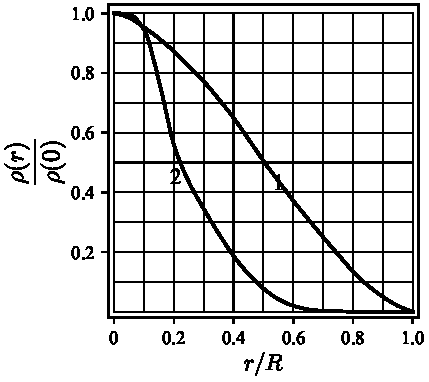
\includegraphics[width=7cm]{fig50.pdf}\\[0.3em]{\small 图 50}\end{minipage}\par\nopagebreak

现在我们来研究由超相对论性的简并电子气所构成的球体的平衡.这种气体的粒子总动能正比于 $N\left(\dfrac NV\right)^{1/3}$（参看(61.3)），也就是正比于 $\dfrac{M^{4/3}}{R}$；而引力势能正比于 $-\dfrac{M^2}{R}$.因此，这两个量以同样的方式依赖于 $R$，而它们的和也具有形式：常数$\cdot R^{-1}$.由此得出结论：一般来讲，物体不可能处于平衡状态：如果常数$>0$，则它有膨胀的趋势，直到气体变成非相对论性时为止；如果常数$<0$，则与总能量的降低相对应的是 $R$ 趋向于0，即物体将无限制地收缩.只有在常数$=0$ 的特殊情形下，物体才可能处于平衡状态，并且是处于 $R$ 为任意值的随遇平衡状态.

这些定性的讨论自然完全被定量的精确分析所证实.所考虑的相对论性气体的化学势同密度的关系为（参看(61.2)）：
\begin{equation}
  \mu=(3\pi^2)^{1/3}\hbar c\left(\frac{\rho}{m'}\right)^{1/3}.
\end{equation}
代替方程式(107.5)，我们现在得到：
\begin{equation}
  \frac{1}{r^2}\frac{\mathrm{d}}{\mathrm{d}r}
  \left(r^2\frac{\mathrm{d}\mu}{\mathrm{d}r}\right)=-\lambda\mu^3,
  \qquad\lambda=\frac{4Gm^{\prime\,2}}{3\pi c^3\hbar^3}.
\end{equation}
现在 $\lambda$ 的量纲为 $\mathrm{erg^{-2}cm^{-2}}$，注意到这一点，我们就发现：化学势作为 $r$ 的函数必须具有形式
\begin{equation}
  \mu(r)=\frac{1}{R\sqrt{\lambda}}f\left(\frac rR\right),
\end{equation}
而密度分布为
\begin{equation*}
  \rho(r)=\frac{\text{常数}}{R^3}F\left(\frac rR\right).
\end{equation*}
因此平均密度现在反比于 $R^3$，而总质量 $M\propto R^3\bar{\rho}$ 是一个与球体大小无关的常数：
\begin{equation}
  \bar{\rho}\propto\frac{1}{R^3},\qquad
  M=\text{常数}\equiv M_0.
\end{equation}
$M_0$ 是平衡成为可能的唯一质量值；当 $M>M_0$ 时，物体有无限收缩的趋势，而当 $M<M_0$ 时，物体膨胀.

要精确地计算“临界质量”$M_0$，必须数值积分(107.14)中函数 $f(\xi)$ 所满足的方程：
\begin{equation}
  \frac{1}{\xi^2}\frac{\mathrm{d}}{\mathrm{d}\xi}
  \left(\xi^2\frac{\mathrm{d}f}{\mathrm{d}\xi}\right)=-f^3,\qquad
  f'(0)=0,\quad f(1)=0.
\end{equation}
我们现在得到：
\begin{equation*}
  f(0)=6.897,\qquad f'(1)=-2.018.
\end{equation*}
对于总质量我们求出：
\begin{equation*}
  GM_0=\left.R^2\frac{\mathrm{d}\varphi}{\mathrm{d}r}\right|_{r=R}
  =-\frac{f'(1)}{m'\sqrt{\lambda}},
\end{equation*}
由此得出
\begin{equation}
  M_0=\frac{3.1}{m^{\prime\,2}}\left(\frac{\hbar c}{G}\right)^{3/2}
  =5.8\left(\frac{m_n}{m'}\right)^2\odot.
\end{equation}
令 $m'=2m_n$，我们得到 $M_0=1.45\odot$.最后，中心密度与平均密度的比值等于
\begin{equation*}
  \frac{\rho(0)}{\bar{\rho}}=-\frac{f^3(0)}{3f'(1)}=54.2.
\end{equation*}
在图 50 中的曲线 2 给出在超相对论性的情形下 $\dfrac{\rho(r)}{\rho(0)}$ 作为 $\dfrac rR$ 的函数\footnote{有关引力气体球平衡时 $P$ 随 $\rho$ 的幂律依赖关系问题由埃姆登（R. Emden，1907）进行了研究. 有关极限质量的存在及其值(107.17)的物理论证由 C.钱德拉塞卡（C. Chandrasekhar，1931）和 Я.Я.朗道（1932）作出.}.

上面所得到的一个结果是关于平衡“冷”球体的质量和半径之间在 $R$ 的整个变化范围内的依赖关系，它可以表示成确定依赖关系的 $M=M(R)$ 单一曲线.当 $R$ 很大（因而物体的密度很小）时，电子气可以看成是非相对论性的，因而函数 $M(R)$ 按 $M\propto R^{-3}$ 的规律下降.当 $R$ 足够小时，密度可以很大，以至于出现超相对论性的情形，这时函数 $M(R)$ 差不多是常数 $M_0$（严格地讲，$R\to0$ 时，$M(R)\to M_0$）.在图 51 中显示了取 $m'=2m_n$ 而计算出来的 $M=M(R)$ 曲线\footnote{曲线的中间部分，通过利用简并气体的精确相对论性物态方程（参看§61习题3）数值积分(107.3)而绘出.}.必须注意到：极限值 1.45$\odot$ 只是渐渐地达到；这是因为密度随着远离物体中心而很快地下降；因此中心附近气体可以已经是超相对论性的，而同时在物体的绝大部分体积内却还是非相对论性的.还应当指出：曲线的开始部分（$R$ 太小）没有实际物理意义.事实上，当半径过小时，密度变得如此之大，以致在物质中开始发生核反应.这时随着密度的增加，压强增长比 $\rho^{4/3}$ 慢，而在这样的物态方程下，一般来讲，任何平衡都是不可能的\footnote{如果化学势正比于密度的某次幂：$\mu\propto\rho^{n}$（因而 $P\propto\rho^{n+1}$），则物体的内能正比于 $V\rho^{n+1}$，亦即 $M^{n+1}/R^{3n}$；而引力势能仍旧正比于 $-M^{2}/R$. 于是很容易看出：当 $n<1/3$ 时，两个这样表达式之和作为 $R$ 的函数虽然也具有极值，但这个极值是极大而不是极小.}.

\par\nopagebreak\noindent\begin{minipage}{\linewidth}\centering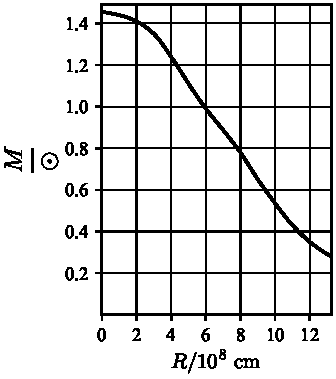
\includegraphics[width=7cm]{fig51.pdf}\\[0.3em]{\small 图 51}\end{minipage}\par\nopagebreak

最后，当 $R$ 值太大（因而 $M$ 太小）时这条曲线也失去意义；如以前所证明的（参看本节第二个脚注），我们用的物态方程在这个范围内已不适用.与此相联系，应当指出：“冷”物体通常可能具有的大小存在上限.事实上，在图 51 中，物体的大线度对应于小质量和小密度.但是当密度足够小时，物质将处于通常的“原子”状态，并且在所考虑的低温下将成为固体.由这样的物质构成的物体，当进一步减少质量时，其大小显然要减小而不会像图 51 那样反而增加.因而 $R=R(M)$ 的实际曲线必然在某一 $M$ 值处有极大.

注意到这个半径的极大值必定对应于电子同核的相互作用变得重要的密度，即
\begin{equation*}
  \rho\sim\left(\frac{m_ee^2}{\hbar^2}\right)^3m'Z^2
\end{equation*}
（参看(106.1)），容易确定半径的数量级.把这个密度式与(107.10)式结合，我们就得到：
\begin{equation}
  R_{\mathrm{max}}\sim
  \frac{\hbar^2}{G^{1/2}em_em'Z^{1/3}}
  \sim10^5\,\frac{m_n}{m'Z^{1/3}}\,\mathrm{km}.
\end{equation}

\section{引力物体的能量}

大家知道，物体的引力势能 $E_{\mathrm{gr}}$ 由下式给出：
\begin{equation}
  E_{\mathrm{gr}}=\frac12\int\rho\varphi\,\mathrm{d}V,
\end{equation}
此处积分遍及物体的整个体积.但是从这个量的另一表达式出发更为方便，它可以用下述方式求得.我们设想：物体是由“取”自无穷远的物质逐渐“构成”的.设 $M(r)$ 是半径为 $r$ 的球内所包含物质的质量.我们假设 $r$ 为某一值的质量 $M(r)$ 已经从无穷远取来；于是为了移送一附加质量 $\mathrm{d}M(r)$ 所需作的功，就等于这一质量（以半径为 $r$ 且厚度为 $\mathrm{d}r$ 的球壳形式分布）在质量 $M(r)$ 的引力场中的势能，即
\begin{equation*}
  -\frac{GM(r)}{r}\,\mathrm{d}M(r).
\end{equation*}
因此半径为 $R$ 的球体其总引力势能为
\begin{equation}
  E_{\mathrm{gr}}=-G\int\frac{M(r)}{r}\,\mathrm{d}M(r).
\end{equation}
把平衡条件(107.2)进行微分，我们得到：
\begin{equation*}
  v\frac{\mathrm{d}P}{\mathrm{d}r}
  +m'\frac{\mathrm{d}\varphi}{\mathrm{d}r}=0
\end{equation*}
（微分必须在恒温下取，$\left(\dfrac{\partial\mu}{\partial P}\right)_T=v$ 是属于一个粒子的体积）.微商 $-\dfrac{\mathrm{d}\varphi}{\mathrm{d}r}$ 是作用于离中心距离为 $r$ 处的单位质量的引力，它等于 $-\dfrac{GM(r)}{r^2}$.再引入密度 $\rho=\dfrac{m'}{v}$，我们就得到：
\begin{equation}
  \frac{1}{\rho}\frac{\mathrm{d}P}{\mathrm{d}r}
  =-\frac{GM(r)}{r^2}.
\end{equation}
根据此式把 $\dfrac{GM(r)}{r}$ 用 $\dfrac{\mathrm{d}P}{\mathrm{d}r}$ 表示，并且记 $\mathrm{d}M(r)=\rho(r)\cdot4\pi r^2\mathrm{d}r$，(108.2)式可表示成
\begin{equation*}
  E_{\mathrm{gr}}=4\pi\int_0^R r^3\frac{\mathrm{d}P}{\mathrm{d}r}\,
  \mathrm{d}r,
\end{equation*}
然后进行分部积分（并考虑到在物体的表面上，$P(R)=0$，并且当 $r\to0$ 时，$r^3P\to0$），得到
\begin{equation*}
  E_{\mathrm{gr}}=-12\pi\int_0^R Pr^2\,\mathrm{d}r,
\end{equation*}
即
\begin{equation}
  E_{\mathrm{gr}}=-3\int P\,\mathrm{d}V.
\end{equation}
因此，平衡物体的引力势能可以表示为它的压强对体积积分的形式.

我们把这个公式应用于上节所考虑的由简并费米气体构成的物体.我们对一般情形计算，并假设物质的化学势正比于密度的某次幂：
\begin{equation}
  \mu=K\rho^{1/n}.
\end{equation}
考虑到：$\mathrm{d}\mu=v\,\mathrm{d}P=\dfrac{m'}{\rho}\,\mathrm{d}P$，得到压强
\begin{equation}
  P=\frac{K}{(n+1)m'}\rho^{1+1/n}.
\end{equation}
在平衡条件
\begin{equation*}
  \frac{\mu}{m'}+\varphi=\text{常数}
\end{equation*}
中，右边的常数就是物体表面上的势，那里 $\mu$ 变成零；这个势等于 $-\dfrac{GM}{R}$（$M=M(R)$ 是物体的总质量），因此可以写：
\begin{equation*}
  \varphi=-\frac{\mu}{m'}-\frac{GM}{R}.
\end{equation*}
把这个式子代入决定引力势能的积分(108.1)，并利用公式(108.5)、(108.6)，我们求出：
\begin{equation*}
  E_{\mathrm{gr}}=-\frac{1}{2m'}\int\mu\rho\,\mathrm{d}V
  -\frac{GM}{2R}\int\rho\,\mathrm{d}V
  =-\frac{n+1}{2}\int P\,\mathrm{d}V-\frac{GM^2}{2R}.
\end{equation*}
最后，根据(108.4)把等式右边的积分用 $E_{\mathrm{gr}}$ 表示，我们就得到：
\begin{equation}
  E_{\mathrm{gr}}=-\frac{3}{5-n}\frac{GM^2}{R}.
\end{equation}
因此，物体的引力势能可以通过它的总质量和半径由一个简单的公式表示出来.

对于物体内部的热能 $E$ 也可以得到一个类似的公式.单粒子的内能等于 $\mu-Pv$（在温度和熵等于零的条件下）；因此单位体积的能量为
\begin{equation*}
  \frac1v(\mu-Pv)=\frac{\rho\mu}{m'}-P=nP
\end{equation*}
（推导后一等式时用了公式(108.5)和(108.6)）.因此整个物体的内能为
\begin{equation}
  E=n\int P\,\mathrm{d}V=-\frac n3E_{\mathrm{gr}}
  =\frac{n}{5-n}\frac{GM^2}{R}.
\end{equation}
最后，物体的总能量为
\begin{equation}
  E_{\mathrm{tot}}=E+E_{\mathrm{gr}}
  =-\frac{3-n}{5-n}\frac{GM^2}{R}.
\end{equation}
对于非相对论性的简并气体，我们有 $n=\dfrac32$，因此\footnote{值得注意：在这种情形下，$2E=-E_{\mathrm{gr}}$，这与力学中按牛顿定律相互作用的粒子系统所适用的位力定理（参看本教程第一卷§10）是一致的.}
\begin{equation}
  E_{\mathrm{gr}}=-\frac67\frac{GM^2}{R},\qquad
  E=\frac37\frac{GM^2}{R},\qquad
  E_{\mathrm{tot}}=-\frac37\frac{GM^2}{R}.
\end{equation}
而在超相对论性的情形下，我们有 $n=3$，因此
\begin{equation}
  E_{\mathrm{gr}}=-E=-\frac32\frac{GM^2}{R},\qquad
  E_{\mathrm{tot}}=0.
\end{equation}
在这种情形下总能量等于0，这与前一节关于这种物体的平衡所作的定性讨论是一致的\footnote{为避免误解，应该提醒：相对论性内能 $E$（因之还有(108.11)中的 $E_{\mathrm{tot}}$）含有（产生压强 $P$ 的）粒子的静止能量. 如果 $E_{\mathrm{tot}}$ 定义为物体的“结合能”（不记散布在空间中的物质的能量），则应该从中扣除粒子的静止能量.}.

\section{中子球体的平衡}

大质量的物体存在两种可能的平衡状态.一种对应于物质的电子-核状态，§107 中数值计算时就是这样假设的.另一种则对应于物质的“中子”状态，那里差不多所有的电子都被质子所俘获，而物质可以看成是中子气体.当物体的质量足够大时，第二种可能性必然变得比第一种在热力学上更为有利（W.Baade，F.Zwicky，1934）.虽然核和电子转变成自由中子有相当大的能量耗费，但是当物体的总质量足够大时，物体由于线度减小和密度增加而释放出的引力能量足以抵消能量耗费.

首先我们来研究这样的问题：在什么条件下物体的中子状态可以有热力学平衡（即便是亚稳定的）.为此，我们从平衡条件
\begin{equation*}
  \mu+m_n\varphi=\text{常数}
\end{equation*}
出发，式中 $\mu$ 为化学势（单中子的热力学势），$m_n$ 为中子质量，$\varphi$ 为引力势.

因为在物体边界处压强必须等于零，显然在物体的某个外层物质有不大的压强和密度，因而处于电子-核状态.虽然这一“壳”层的厚度也会与内部稠密的中子“核心”的半径可比，但是由于这一层的密度很小，可以认为它的总质量比核心的质量小得多\footnote{自然，在“核心”和“壳”之间并没有任何显著的边界存在，它们之间以连续的方式过渡.}.

我们在两个位置即稠密核心边界附近和壳的外边界附近，比较它们的 $\mu+m_n\varphi$.在这两点的引力势可以认为各等于 $-\dfrac{GM}{R}$ 和 $-\dfrac{GM}{R'}$，其中 $R$ 和 $R'$ 分别为核心和壳的半径，而 $M$ 为核心的质量，在我们所作的近似下等于物体的总质量.至于化学势，则在这两种情形下主要都决定于相应粒子的内能（结合能），它们比热能要大得多.因此可以令这两个化学势之差就等于每单位原子量的中性原子（即核和 $Z$ 个电子）的静止能量和中子静止能量之差；这个量用 $\Delta$ 表示.因此令 $\mu+m_n\varphi$ 之值在所考虑的两个位置的值相等，我们就得到：
\begin{equation*}
  m_nMG\left(\frac1R-\frac{1}{R'}\right)=\Delta.
\end{equation*}
由此可以看出：不论半径 $R'$ 的值如何，中子核心的质量和半径都必须满足不等式
\begin{equation}
  \frac{m_nMG}{R}>\Delta.
\end{equation}
从另一方面来看，把§107的结果应用于由（非相对论性）简并中子气体构成的球体，可知 $M$ 和 $R$ 彼此联系如下式：
\begin{equation}
  MR^3=91.9\,\frac{\hbar^6}{G^3m_n^8}
  =3.6\times10^3\odot\,\mathrm{km}^3
\end{equation}
（即(107.10)式，但式中 $m_e$ 和 $m'$ 应改为 $m_n$）.由此把 $M$ 用 $R$ 来表示并代入(109.1)，我们就得到关于 $M$ 的不等式.其数值估计为：
\begin{equation*}
  M>\sim0.2\odot.
\end{equation*}
例如，取氧的 $\Delta$ 值，则我们得到 $M>0.17\odot$，对铁则 $M>0.18\odot$.这样的质量相当于半径 $R<26\,\mathrm{km}$\footnote{值得强调：本节中的数值估算基于对物质结构的简单假设，不应该赋予过分的直接天体物理学涵义.}.

所得到的这个不等式确定了一个质量下限，低于它时物体的中子状态绝不可能稳定.但是它并不保证状态的完全稳定性，状态也可能是亚稳的.为了确定亚稳性的界限，必须比较物体在中子状态和电子-核状态的总能量.从一方面来讲，整个质量 $M$ 从电子-核状态转变到中子状态要求损耗能量
\begin{equation*}
  \frac{M}{m_n}\Delta
\end{equation*}
以补偿核结合能.从另一方面来讲，这时由于物体的收缩发生能量的释放；根据公式(108.10)，这一能量增益等于
\begin{equation*}
  \frac{3GM^2}{7}\left(\frac{1}{R_n}-\frac{1}{R_e}\right),
\end{equation*}
式中 $R_n$ 为物体在中子状态的半径，由公式(109.2)所确定；$R_e$ 为物体在电子-核状态的半径，由公式(107.10)确定.因为 $R_e\gg R_n$，所以可略去 $\dfrac{1}{R_e}$，我们得到如下保证物体的中子状态完全稳定的条件（省略掉 $R_n$ 的角标）：
\begin{equation}
  \frac{3GMm_n}{7R}>\Delta.
\end{equation}
把这个条件同条件(109.1)进行比较，并考虑(109.2)，我们就看到：由不等式(109.3)所确定的下限质量高于由(109.2)所得值达 $\left(\dfrac73\right)^{3/4}=1.89$ 倍.因此，中子状态的亚稳性界限数值上位于质量
\begin{equation*}
  M\approx\frac13\odot
\end{equation*}
（而半径 $R\approx22\,\mathrm{km}$）\footnote{这时物体的平均密度等于 $1.4\times10^{13}\,\mathrm{g/cm^{3}}$，因此中子气体实际上仍旧可以认为是非相对论性的，而上面所用的各式仍旧适用.}.

现在我们来讨论中子物体仍有平衡状态的质量值上限问题.假如我们应用§107的结果（公式(107.17)，但以 $m_n$ 代替 $m'$），那么我们就会得到这个上限值为 6$\odot$.但是实际上，§107的结果并不适用于这里所考虑的情形，原因如下：在相对论性的中子气体中，粒子的动能与静止能量同数量级（或更大）\footnote{在相对论性的电子气中，粒子的动能虽然与电子的静止能量同数量级，但是同构成物质主要质量的核的静止能量相比仍旧很小.}，而引力势 $\varphi\sim c^2$.由于这个缘故，牛顿引力理论已变得不适用，而必须根据广义相对论来进行计算.同时我们在下面将会看到，超相对论性的情形是根本达不到的；因此必须用简并费米气体的精确物态方程（见§61的习题3）来进行计算.

数值积分中心对称的静引力场方程完成计算，可得结果如下\footnote{关于计算的细节，可参看原始文献 Oppenheimer J R, Volkoff G M. Phys. Rev., 1939, 55: 374.}：平衡中子球体质量的极限值只不过 $M_{\mathrm{max}}=0.76\odot$，并且这个值在有限的半径（等于 $R_{\mathrm{min}}=9.42\,\mathrm{km}$）下就已经达到；在图 52 描绘了所得到的质量 $M$ 对半径 $R$ 的依赖关系曲线.因此，质量更大或半径更小的稳定中子球体不可能存在.

\par\nopagebreak\noindent\begin{minipage}{\linewidth}\centering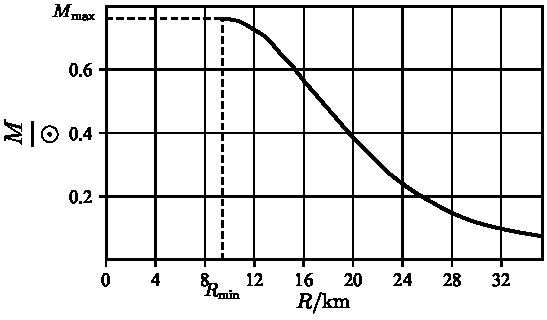
\includegraphics[width=7cm]{fig52.pdf}\\[0.3em]{\small 图 52}\end{minipage}\par\nopagebreak

应该指出：这里的质量 $M$ 我们理解为乘积 $M=Nm_n$，式中 $N$ 为球体中粒子（中子）的总数.这个质量与决定物体在周围空间产生引力场的引力质量 $M_{\mathrm{gr}}$ 并不一致.由于“引力质量亏损”的缘故，在稳定状态下始终有 $M_{\mathrm{gr}}<M$（例如，在 $R=R_{\mathrm{min}}$ 时，$M_{\mathrm{gr}}=0.95M$）\footnote{图 52 中的点 $R=R_{\mathrm{min}}$ 实际上是曲线 $M=M(R)$ 的极大点. 该曲线以螺线的形式延伸至极大点外，渐近地趋于某个中心. 球心的密度是沿整条曲线单调递增的参量，对于与螺线极限点对应的球体，它趋向于无穷大（Н. А. Дмитриев，С. А. Холин，1963）. 但是曲线在 $R<R_{\mathrm{min}}$ 的部分并不对应于球的稳定态.\par\noindent
相应的研究参看 Дмитриев Н А, Холин С Л. Вопросы космогонии, 1963, 9; Гаррисон Б К, Торн К С, Вакано М, Уилер Дж А. Теория гравитации и гравитационный коллапс. М.: Мир, 1967（Harrison B K, Thorne K S, Wakano M, Wheeler J A. Gravitation Theory and Gravitational Collapse. Chicago: University of Chicago Press, 1965）.}.

至于质量超过 $M_{\mathrm{max}}$ 时球体的性状问题，事先可知，它将趋向于无限地收缩.

这种无限制的引力坍缩的特点在本教程的另一卷中研究（参看第二卷§102—§104）.

在 $M>M_{\mathrm{max}}$ 时（对于所考虑的球体模型）引力坍缩必不可免，应当指出，这种坍缩的大体可能性实际上并不限于大质量.“坍缩的”状态对于任何质量都存在，但是在 $M<M_{\mathrm{max}}$ 时，它被非常高的势垒与静止平衡状态隔开\footnote{参看 Зельдович Я Б. ЖЭТФ, 1962, 42: 641.}.
